%% =====================================================================
%% Query-Conditioned Budget-Aware Evidence Allocation for RAG  (CS787)
%% Redesigned paper: main body (through Conclusion) <= 8 pages,
%% then References + Appendix.  Compile: pdflatex x2 (no BibTeX needed).
%% =====================================================================
\documentclass[10pt,twocolumn,letterpaper]{article}
\usepackage[top=0.70in,bottom=0.78in,left=0.72in,right=0.72in,columnsep=0.24in]{geometry}
\usepackage[T1]{fontenc}
\usepackage[utf8]{inputenc}
\usepackage{amsmath}
% newtx (Times-like) on Overleaf; falls back to mathptmx if newtx is not installed
\IfFileExists{newtxtext.sty}{\usepackage{newtxtext}\usepackage{newtxmath}}{\usepackage{mathptmx}}
\usepackage{microtype,booktabs,multirow,array,tabularx,graphicx,xcolor,xspace,enumitem,caption,titlesec,fancyhdr,hyperref,cite,float}
\usepackage{tikz,pgfplots}
\usepgfplotslibrary{groupplots}
\usetikzlibrary{positioning,fit,arrows.meta,calc,backgrounds}
\pgfplotsset{compat=1.18}
\usepackage[skins,breakable]{tcolorbox}

% ---------- colours (one colour per method, used consistently) ----------
\definecolor{cblue}{RGB}{31,78,121}     % QBGF
\definecolor{corange}{RGB}{192,101,26}  % BEA-V1
\definecolor{cgreen}{RGB}{46,125,79}    % BEA-V2
\definecolor{cpurple}{RGB}{106,76,147}  % MiniLM cross-encoder
\definecolor{cgray}{RGB}{90,98,110}     % sentence baseline / neutral
\definecolor{cred}{RGB}{170,52,52}
\hypersetup{colorlinks=true,linkcolor=cblue,citecolor=cgreen,urlcolor=cblue}

% ---------- layout ----------
\setlength{\parindent}{0.9em}\setlength{\parskip}{0pt}
\captionsetup{font=footnotesize,labelfont=bf,skip=3pt}
\titleformat{\section}{\normalsize\bfseries\scshape}{\thesection}{0.5em}{}
\titleformat{\subsection}{\normalsize\bfseries}{\thesubsection}{0.5em}{}
\titlespacing*{\section}{0pt}{8pt plus 2pt minus 2pt}{3pt}
\titlespacing*{\subsection}{0pt}{5pt plus 1pt minus 1pt}{2pt}
\titlespacing*{\subsubsection}{0pt}{3pt}{1pt}
\setlength{\textfloatsep}{8pt plus 2pt minus 2pt}\setlength{\floatsep}{6pt plus 2pt minus 2pt}
\setlength{\intextsep}{6pt plus 2pt minus 2pt}\setlength{\dbltextfloatsep}{8pt plus 2pt minus 2pt}
\setlength{\abovedisplayskip}{4pt}\setlength{\belowdisplayskip}{4pt}
\setlength{\abovedisplayshortskip}{2pt}\setlength{\belowdisplayshortskip}{2pt}
\setcounter{topnumber}{4}\setcounter{dbltopnumber}{4}
\renewcommand{\topfraction}{0.95}\renewcommand{\dbltopfraction}{0.95}
\renewcommand{\textfraction}{0.04}\renewcommand{\floatpagefraction}{0.80}\renewcommand{\dblfloatpagefraction}{0.80}
\setlist[itemize]{leftmargin=1.2em,noitemsep,topsep=1.5pt,parsep=0pt}
\setlist[enumerate]{leftmargin=1.3em,noitemsep,topsep=1.5pt,parsep=0pt}
\pagestyle{fancy}\fancyhf{}
\fancyhead[L]{\footnotesize CS787 course project report}
\fancyhead[R]{\footnotesize IIT Kanpur}
\fancyfoot[C]{\footnotesize\thepage}
\renewcommand{\headrulewidth}{0.3pt}

% ---------- macros ----------
\newcommand{\qbgf}{\textsc{QBGF}\xspace}
\newcommand{\vone}{\textsc{BEA-V1}\xspace}
\newcommand{\vtwo}{\textsc{BEA-V2}\xspace}
\newcommand{\hotpot}{\textsc{HotpotQA}\xspace}
\newcommand{\qasper}{\textsc{QASPER}\xspace}
\newcommand{\scifact}{\textsc{SciFact}\xspace}
\newcommand{\Phelp}{P_{\mathrm{help}}}
\newcommand{\SmallTable}{\footnotesize\setlength{\tabcolsep}{3.6pt}}
\newtcolorbox{case}[2][]{enhanced,breakable,colback=#2!5,colframe=#2!70!black,boxrule=0.5pt,arc=1.5pt,
  left=3pt,right=3pt,top=2pt,bottom=2pt,fontupper=\footnotesize,fonttitle=\footnotesize\bfseries,#1}
\newtcolorbox{apbox}[1][]{enhanced,breakable,colback=black!3,colframe=black!55,boxrule=0.5pt,arc=1.5pt,
  left=3pt,right=3pt,top=2pt,bottom=2pt,fontupper=\footnotesize,fonttitle=\footnotesize\bfseries,#1}

% ---------- TikZ styles ----------
\tikzset{
  box/.style={draw=#1!70!black,fill=#1!8,rounded corners=1.5pt,align=center,inner sep=2.5pt,font=\scriptsize,line width=0.5pt},
  box/.default=cgray,
  arr/.style={-{Stealth[length=1.7mm,width=1.3mm]},line width=0.6pt,draw=black!65},
}
% one sentence square for Fig. 2: \sq{x}{y}{star?}{fill}
\newcommand{\sq}[4]{\draw[draw=black!50,fill=#4,line width=0.3pt] (#1,#2) rectangle ++(1,1);%
  \ifnum#3=1\node[font=\scriptsize] at (#1+0.5,#2+0.5){$\star$};\fi}

\begin{document}
\twocolumn[{%
\begin{center}
{\LARGE\bfseries Query-Conditioned Budget-Aware Evidence Allocation\\[1pt] for Retrieval-Augmented Generation\par}
\vspace{5pt}
{\large\bfseries Doddi Guna Venkat (251140009)\quad Gagan Kumar Soni (252040606)\par}
\vspace{2pt}
{\small CS787: Generative Artificial Intelligence $\cdot$ Indian Institute of Technology Kanpur\par}
{\small Code and experiment records: \href{https://github.com/Guna-Venkat/QC-BEA-for-RAG}{github.com/Guna-Venkat/QC-BEA-for-RAG}\par}
\end{center}
\vspace{2pt}\hrule\vspace{5pt}
\begin{minipage}{\textwidth}\small
\noindent\textbf{Abstract.}
Retrieval-augmented generation (RAG) often retrieves more text than a reader can use within a fixed evidence-token budget, so a system must decide which retrieved material to show and in what form. Starting from SARA's split between readable and latent evidence, we ask whether the amount of readable context should adapt to the query. Retrospective oracles show large headroom, but learned controllers fail to predict it and under-allocate. Controlled text-only experiments on HotpotQA, QASPER and SciFact then separate passage identity, retrieval, reader-interface effects and evidence granularity. We propose QBGF (Query-Conditioned Budgeted Granularity Fusion), which decides for every retrieved passage whether to drop it, keep a few relevant sentences or keep it whole, by exactly solving a multiple-choice knapsack over a relevance surrogate. Query conditioning helps, yet QBGF does not reliably beat a simple sentence baseline, so a pre-specified rule keeps the sentence baseline for reserved confirmation. Leave-one-out (LOO) interventions show that dense relevance is only weakly aligned with a unit's effect on the reader. This motivates BEA-V1, an incremental allocator that can starve the context by stopping early, and BEA-V2, which weights marginal gains with a classifier trained on historical LOO helpfulness. In exploratory matched comparisons BEA-V2 attains the highest HotpotQA F1 at 256 and 1024 tokens (0.4352 and 0.4234, versus 0.3661 and 0.3893 for sentence selection), but results on QASPER and SciFact are mixed and none of the BEA results is independently confirmed. Exact optimization of relevance is not the same as estimating downstream utility.\par
\end{minipage}
\vspace{5pt}\par
\begin{minipage}{\textwidth}\centering
\newcommand{\stage}[6]{%
 \node[draw=#4,fill=#4,text=white,font=\scriptsize\bfseries,minimum width=4.2cm,minimum height=0.42cm,anchor=north west,inner sep=2pt,align=left] (#1h) at (#2,#3) {#5};
 \node[draw=#4,fill=#4!6,font=\scriptsize,text width=4.0cm,minimum width=4.2cm,minimum height=1.95cm,anchor=north west,inner sep=2pt,align=left] (#1) at (#1h.south west) {#6};}
\begin{tikzpicture}
\stage{s1}{0}{0}{cgray}{1\;\;SARA starting point}{\emph{Question:} can the amount of readable text depend on the query? Static $k{=}5$ (readable of $n{=}10$): F1 0.3629 (\qasper dev, Mistral specialist).}
\stage{s2}{4.55}{0}{cgray}{2\;\;Adaptive context size}{Oracle best-$k$: 0.5008 vs.\ 0.3950 (static $k{=}8$). Learned controllers: 0.30--0.38. False stops cost $2.5\times$ more than false expansions. $\Rightarrow$ \emph{which} evidence?}
\stage{s3}{9.10}{0}{cgray}{3\;\;Identity and granularity}{Same $k{=}4$: 0.391 vs.\ 0.360 by passage choice. At 256 tokens sentences lead (0.421 vs.\ 0.338); passages catch up at 512--1024. $\Rightarrow$ choose fidelity per source.}
\stage{s4}{13.65}{0}{cblue}{4\;\;QBGF}{Exact knapsack over DROP / SENT / FULL per passage. Query conditioning: $+0.02$ to $+0.19$ F1 over no-query; not reliably better than sentences $\Rightarrow$ sentence policy locked.}
\stage{s5}{0}{-3.35}{cred}{5\;\;LOO diagnosis}{Delete one selected unit, regenerate. 70--99\% of units are neutral; $\rho$(relevance, utility) $\le0.13$. Relevance $\neq$ downstream utility.}
\stage{s6}{4.55}{-3.35}{corange}{6\;\;BEA-V1}{Incremental gain per token (relevance, coverage, redundancy) with early stopping. Failure: context starvation (245 of 1024 tokens used; F1 0 on one case).}
\stage{s7}{9.10}{-3.35}{cgreen}{7\;\;BEA-V2}{Gain $\times$ $\Phelp$, learned from historical LOO labels. Exploratory: best \hotpot F1 at both budgets (0.435, 0.423); mixed elsewhere.}
\stage{s8}{13.65}{-3.35}{black}{Evidence status}{Locked and confirmed: sentence baseline beats no evidence in 4/4 cells; \scifact-256 $+0.288$ over passages. BEA-V2 is exploratory and does not overturn the lock.}
\foreach \a/\b in {s1/s2,s2/s3,s3/s4,s5/s6,s6/s7,s7/s8}{\draw[arr] (\a.east) -- (\b.west);}
\draw[arr] (s4.south) -- ++(0,-0.27) -| (s5h.north);
\end{tikzpicture}
\captionof{figure}{Research journey. Each stage records what was learned and why the next experiment followed (grey: historical and diagnostic stages; blue: first proposed allocator; red: diagnosis; orange/green: BEA). Scores come from different tiers (Table~\ref{tab:tiers}) and are not one leaderboard.}\label{fig:journey}
\end{minipage}
\vspace{4pt}\hrule\vspace{6pt}
}]

%=====================================================================
\section{Introduction}\label{sec:intro}
Retrieval-augmented generation (RAG) conditions a language model on retrieved text~\cite{lewis2020rag}, but the retrieved pool is usually larger than the reader can use well: long contexts cost more and are not used uniformly~\cite{liu2024lost}. In our retained exploratory sample of 450 SFR top-10 pools, the mean pool holds 1,375 (\hotpot), 2,458 (\qasper) and 3,322 (\scifact) Qwen tokens, and 83\%, 100\% and 100\% of them exceed a 1,024-token evidence budget (Fig.~\ref{fig:problem}). Something must be left out, and what is left out is often decisive.

\paragraph{A concrete failure.} A \hotpot question asks which film earned the screenwriter of Denis Villeneuve's \emph{Enemy} a Goya nomination for Best Adapted Screenplay. The answer, \emph{Invader (Invasor)}, sits in one 56-token sentence of a second source. In a recorded 256-token run, an incremental allocator that had already spent 168 tokens on short title fragments and unrelated film details rejected that sentence and answered \emph{Enemy}; an allocator that selected it first answered correctly (Appendix~\ref{app:examples}).

\paragraph{Research question.} \emph{Given a limited evidence-token budget, how should we decide which retrieved information to give the reader, in what representation, and according to what notion of usefulness?} We separate four coupled choices: the \emph{quantity} of readable evidence, the \emph{identity} of the sources kept, the \emph{granularity} (whole passage, a few sentences, or nothing) used for each, and the \emph{utility} signal that justifies the choice.

\paragraph{How the project unfolded.} Figure~\ref{fig:journey} is a one-page summary. We started from SARA (Selective and Adaptive RAG)~\cite{jin2026sara}, which keeps $k$ of $n$ retrieved passages as readable text and compresses the rest into latent vectors, and asked whether $k$ should depend on the query. A retrospective oracle says yes; learned controllers could not find the right $k$. At fixed $k$, \emph{which} passages are kept mattered, and the best evidence \emph{unit} depended on the budget. This led to QBGF, which assigns a representation to each passage under one exact budget. QBGF's query conditioning helped but it did not reliably beat a simple sentence baseline; leave-one-out (LOO) interventions suggested why: relevance is weakly aligned with a unit's effect on the reader. BEA-V1 and BEA-V2 (Budgeted Evidence Allocator) are our attempts to allocate by marginal and then by learned utility.

\paragraph{Core insight.} Exact optimization of a relevance score cannot compensate for a mismatch between relevance and what the reader actually needs. QBGF's dynamic program is optimal for its relevance surrogate, but that surrogate is not downstream answer quality.

\paragraph{Contributions.}
\begin{enumerate}
\item \textbf{Where adaptive context fails.} A retrospective best-$k$ oracle reaches 0.5008 F1 versus 0.3950 for static $k{=}8$, yet learned controllers score 0.30--0.38; we then isolate passage identity, retrieval and reader-interface confounds and a budget-dependent (descriptive) granularity pattern.
\item \textbf{QBGF.} An exact multiple-choice knapsack over per-passage fidelities. Query conditioning improves it by 0.020--0.187 F1 over its no-query ablation, but it fails a pre-specified noninferiority rule against sentence selection in five of six cells; the sentence baseline is locked and confirmed.
\item \textbf{Relevance is not utility.} LOO deletions show that most selected units are neutral and that dense relevance correlates weakly with deletion utility ($\rho\le0.134$ in six representative conditions), including a highly relevant unit whose removal fixes a wrong answer.
\item \textbf{BEA-V1/V2 with explicit evidence boundaries.} V1 exhibits context starvation; V2 weights gains by a learned helpfulness probability and, in exploratory matched runs, leads \hotpot by $+0.069$ and $+0.034$ F1 over sentence selection while remaining mixed on \qasper and \scifact. We separate development, validation, locked-selection, confirmation and exploratory evidence throughout.
\end{enumerate}



%=====================================================================
\section{Related Work}\label{sec:related}
\textbf{Compression and selection.} RECOMP~\cite{recomp2024} trains extractive and abstractive compressors, including the option to prepend nothing; our sentence baseline is \emph{not} its trained compressor and we report no matched RECOMP score. SARA~\cite{jin2026sara} mixes readable passages with latent compressed ones; LLMLingua-2~\cite{pan2024llmlingua2} learns token-level retention (we qualified a checkpoint but ran no matched quality comparison). \textbf{Granularity.} Dense X Retrieval~\cite{chen2024densex} studies retrieval units from passages to propositions; our units are exact source sentences and spans. \textbf{Budgeted selection.} Self-Correcting RAG~\cite{xu2026selfcorrecting} combines a knapsack-style selection with NLI-guided search; QBGF's contribution is not dynamic programming but a single-budget, within-source fidelity menu and its controlled analysis. \textbf{Adaptive and reranking baselines.} Adaptive-RAG~\cite{jeong2024adaptive} routes strategies by question complexity; a cross-encoder MS-MARCO MiniLM reranker~\cite{minilmreranker} is the conventional relevance comparator that we pack under the same budgets. None of these external methods is locally reproduced unless stated.

%=====================================================================
\section{Problem Formulation and Evaluation Protocol}\label{sec:problem}
Let $q$ be a query, $\mathcal D=\{p_1,\dots,p_K\}$ the retrieved pool and $E$ the evidence shown to a frozen reader. Ideally
\begin{equation}
E^\star=\arg\max_{E}\ \mathrm{Quality}\bigl(\mathrm{Reader}(q,E)\bigr)\quad\text{s.t.}\quad |\mathrm{Tok}(E)|\le B,\label{eq:ideal}
\end{equation}
but quality is unknown before generation, so every allocator optimizes a \emph{surrogate} (relevance, redundancy, predicted utility). $B\in\{256,1024\}$ bounds \emph{input evidence} tokens only (not instructions, chat framing or the answer); costs are measured on serialized Qwen token-ID blocks including separators.

\begin{figure}[t]\centering
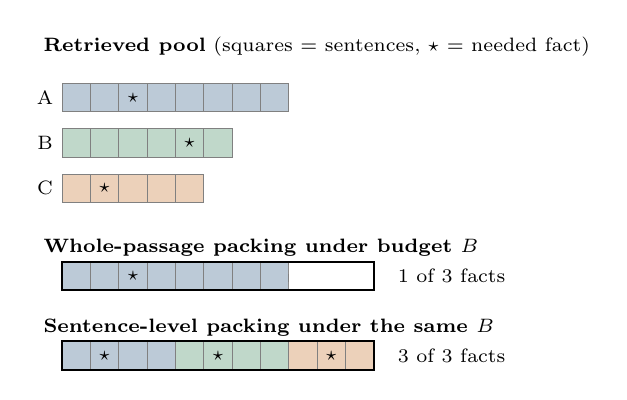
\begin{tikzpicture}[x=0.36cm,y=0.36cm,font=\scriptsize]
\node[anchor=west] at (-1.0,9.3) {\textbf{Retrieved pool} (squares = sentences, $\star$ = needed fact)};
\node at (-0.6,7.5){A};\node at (-0.6,5.9){B};\node at (-0.6,4.3){C};
\foreach \i in {0,...,7}{\pgfmathtruncatemacro{\st}{\i==2?1:0}\sq{\i}{7}{\st}{cblue!30}}
\foreach \i in {0,...,5}{\pgfmathtruncatemacro{\st}{\i==4?1:0}\sq{\i}{5.4}{\st}{cgreen!30}}
\foreach \i in {0,...,4}{\pgfmathtruncatemacro{\st}{\i==1?1:0}\sq{\i}{3.8}{\st}{corange!30}}
\node[anchor=west,font=\scriptsize\bfseries] at (-1.0,2.2) {Whole-passage packing under budget $B$};
\foreach \i in {0,...,7}{\pgfmathtruncatemacro{\st}{\i==2?1:0}\sq{\i}{0.7}{\st}{cblue!30}}
\draw[dashed,black!45] (8,0.7) rectangle (11,1.7);
\draw[line width=0.8pt] (0,0.7) rectangle (11,1.7);
\node[anchor=west,font=\scriptsize] at (11.5,1.2) {1 of 3 facts};
\node[anchor=west,font=\scriptsize\bfseries] at (-1.0,-0.6) {Sentence-level packing under the same $B$};
\sq{0}{-2.1}{0}{cblue!30}\sq{1}{-2.1}{1}{cblue!30}\sq{2}{-2.1}{0}{cblue!30}\sq{3}{-2.1}{0}{cblue!30}
\sq{4}{-2.1}{0}{cgreen!30}\sq{5}{-2.1}{1}{cgreen!30}\sq{6}{-2.1}{0}{cgreen!30}\sq{7}{-2.1}{0}{cgreen!30}
\sq{8}{-2.1}{0}{corange!30}\sq{9}{-2.1}{1}{corange!30}\sq{10}{-2.1}{0}{corange!30}
\draw[line width=0.8pt] (0,-2.1) rectangle (11,-1.1);
\node[anchor=west,font=\scriptsize] at (11.5,-1.6) {3 of 3 facts};
\end{tikzpicture}
\caption{The allocation problem (illustrative schematic, not measured data). With the same budget, whole passages fill it with one long source, while sentence units can cover several sources; passages instead preserve local context. Which wins depends on the budget and task.}\label{fig:problem}
\end{figure}

\paragraph{Pipeline, tasks and metrics.} SFR-Embedding-Mistral retrieves the top-10 passages and base Qwen3-8B (FP16, greedy decoding, no LoRA) reads the selected evidence. \hotpot is used in its 10-paragraph distractor setting; \qasper is scientific-paper QA; \scifact is claim verification with exact labels (\texttt{SUPPORT}, \texttt{REFUTE}, \texttt{NOT\_ENOUGH\_INFO}). \hotpot and \qasper use Answer F1, \scifact uses three-class macro-F1; scores are never pooled across tasks and invalid labels count as wrong.

\paragraph{Evaluation tiers.} Experiments differ in cohort, reader and retrieval interface, so we do not merge them into one leaderboard (Table~\ref{tab:tiers}).

\begin{table*}[t]\centering\SmallTable
\caption{Evaluation tiers. Only the validation, locked rule and reserved confirmation tiers support selection and generalization claims; LOO/BEA results are exploratory.}\label{tab:tiers}
\begin{tabularx}{\textwidth}{@{}p{3.15cm}p{5.0cm}p{3.5cm}X@{}}\toprule
Tier & Cohort & Reader / retrieval & Used for\\\midrule
SARA development (\S\ref{sec:evolution}) & \qasper, 231 questions / 86 papers & adapted Mistral-7B specialist, BM25 & oracles, controllers, passage identity\\
Granularity pilot (\S\ref{sec:evolution}) & \hotpot dev, 50 queries & Qwen3-8B, SFR & granularity vs.\ budget\\
Full validation (\S\ref{sec:qbgf}) & 8,337 queries: \hotpot 7,155; \qasper 1,005 (281 papers); \scifact 177 (157 groups) & Qwen3-8B, SFR & QBGF, ablations, locked rule\\
Reserved confirmation (\S\ref{sec:qbgf}) & \hotpot 200; \scifact 50 (43 groups); no \qasper & Qwen3-8B, SFR & test of the locked policy\\
Exploratory LOO / BEA (\S\ref{sec:loo}--\ref{sec:bea}) & 50 queries per dataset (150), development data that overlap validation & Qwen3-8B, SFR & LOO, BEA-V1/V2, MiniLM; \emph{not} confirmation\\\bottomrule
\end{tabularx}\end{table*}

%=====================================================================
\section{From SARA to Evidence Granularity}\label{sec:evolution}
\subsection{Starting point: readable versus latent evidence}
SARA (Fig.~\ref{fig:sara}) keeps $k$ of the $n{=}10$ retrieved passages as readable text and turns the others into learned soft tokens. Our specialist uses Mistral-7B-Instruct with a Mistral-specific projector and LoRA, so it is \emph{not} a drop-in component for later Qwen experiments, and its scores are not matched to the Qwen budgeted pipeline. Static $k{=}5$ reaches F1 0.3629 (EM 0.1861; 1,157 mean context tokens) on our 231-question \qasper development cohort; quality rises with $k$ (0.1388 at $k{=}0$, 0.3950 at $k{=}8$, 0.4090 at $k{=}10$). Note that $k{=}0$ still supplies latent evidence and is not a no-evidence baseline.

\begin{figure}[t]\centering
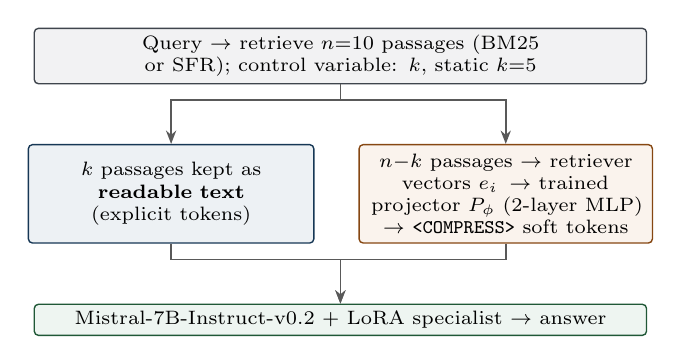
\begin{tikzpicture}[font=\scriptsize]
\node[box=cgray,text width=7.6cm] (q) at (0,0) {Query $\to$ retrieve $n{=}10$ passages (BM25 or SFR); control variable: $k$, static $k{=}5$};
\node[box=cblue,text width=3.45cm,minimum height=1.25cm] (l) at (-2.15,-1.75) {$k$ passages kept as\\\textbf{readable text}\\(explicit tokens)};
\node[box=corange,text width=3.55cm,minimum height=1.25cm] (r) at (2.1,-1.75) {$n{-}k$ passages $\to$ retriever vectors $e_i\to$ trained projector $P_\phi$ (2-layer MLP) $\to$ \texttt{<COMPRESS>} soft tokens};
\node[box=cgreen,text width=7.6cm] (m) at (0,-3.35) {Mistral-7B-Instruct-v0.2 + LoRA specialist $\to$ answer};
\draw[arr](q.south)--++(0,-0.2)-|(l.north);\draw[arr](q.south)--++(0,-0.2)-|(r.north);
\draw[arr](l.south)--++(0,-0.2)-|(m.north);\draw[arr](r.south)--++(0,-0.2)-|(m.north);
\end{tikzpicture}
\caption{SARA-inspired starting point (initial specialist setting). The projector and LoRA were trained for Mistral; the later Qwen3-8B studies are text-only and use no latent path.}\label{fig:sara}
\end{figure}

\subsection{Adaptive context size: headroom without a predictor}
A retrospective oracle picks, for each question, the $k$ with the best outcome \emph{after} seeing answer quality. Over $k\le8$ it reaches F1 0.5008 ($+26.8\%$ over static $k{=}8$), and a cost-aware oracle reaches 0.4894 at mean $k{=}3.49$ using 841 instead of 1,759 tokens (Fig.~\ref{fig:early}a). Questions really disagree (box below), but the oracle uses outcomes: it is a ceiling, not a policy.

\begin{case}[title={Example: two questions, opposite context needs}]{cgray}
Both questions come from one \qasper paper (SARA specialist). \emph{Q1} (``Which psycholinguistic and basic linguistic features are used?'') is decided by the rank-6 passage: F1 0.133 at $k{=}0$, 0.143 at $k{=}2$--5, \textbf{0.600} at $k{=}6$, then 0.417 ($k{=}8$) and 0.348 ($k{=}10$). \emph{Q2} (Twitter vs.\ Facebook communication styles) is best with no explicit passage: 0.250 at $k{=}0$, 0.200 at $k{=}10$ (Appendix~\ref{app:examples}).
\end{case}

\paragraph{Why prediction failed.} Sixty-four pre-generation features (query complexity, retrieval-score structure, redundancy, coverage) had no association with the oracle $k$ that survived FDR correction ($q{=}0.10$). A flat logistic controller fell to 0.3034 F1 at mean $k{=}2.03$; a sequential $2{\to}4{\to}6{\to}8$ controller was unpredictable at the first step (ROC-AUC 0.439) and modest at $4{\to}6$ (0.650); the best balanced logistic policy reached 0.3842. The obstacle is \emph{asymmetric cost}: a useful expansion gained $+0.3395$ F1 on average, an unnecessary one cost $-0.1345$ ($2.5\times$ less). Conservative controllers therefore dropped decisive evidence, while recall-preserving ones drifted back to full context: a content-aware controller matched static $k{=}8$ (0.3952 vs.\ 0.3950) only at mean $k{=}7.85$, saving 1.72\% of tokens. \emph{Lesson: choosing how much evidence is insufficient if we do not choose the right evidence.}

\subsection{Identity, retrieval and reader interface}
At fixed $k{=}4$ on one candidate pool, dense semantic routing reached 0.3913 F1 versus 0.3596 (retrieval order) and 0.3572 (learned ranker) (Fig.~\ref{fig:early}b), so identity matters at unchanged quantity (a worked case in Appendix~\ref{app:examples} shows only the route containing a rank-8 passage names the language pair). Before attributing differences to allocation we checked confounds. Top-10 any-evidence recall was 0.618 (BM25), 0.636 (MiniLM bi-encoder) and 0.727 (SFR). With SFR fixed at $k{=}6$, full-text RAG (0.4199) and SARA's text-plus-latent mixture (0.4213) were indistinguishable (paired interval crossing zero), so latent compression could not be credited with earlier gains. On \scifact, strict-label parsing exposed an interface confound: of 1,850 conditions per reader, Mistral produced 1,849 invalid outputs and Llama 1,826 (often a correct label followed by an explanation), versus none for Qwen. These are interface measurements, not reasoning rankings; we kept Qwen3-8B as the controlled reader and compared textual evidence directly. Learned utility routers, draft-promotion gates and generative extraction (below its own no-intervention reference) gave no consistent gain (Appendix~\ref{app:early}).

\subsection{Granularity depends on the budget}
Holding SFR and Qwen fixed, a 50-query \hotpot pilot compared whole passages, exact sentences and finer spans at 256/512/1,024 tokens (Fig.~\ref{fig:early}c). At 256 tokens sentences led passages by $+0.084$ F1 (0.421 vs.\ 0.338, $+24.8\%$), plausibly because smaller units spread a tight budget over more sources (not isolated causally); at 512 and 1,024 tokens passages had the highest point estimates (0.456, 0.480). Interaction intervals crossed zero, so this is a descriptive pattern, not a law. It motivates the next question: \emph{instead of one unit size for all passages, can we choose a fidelity for each source under a shared budget?}

\begin{figure*}[t]\centering
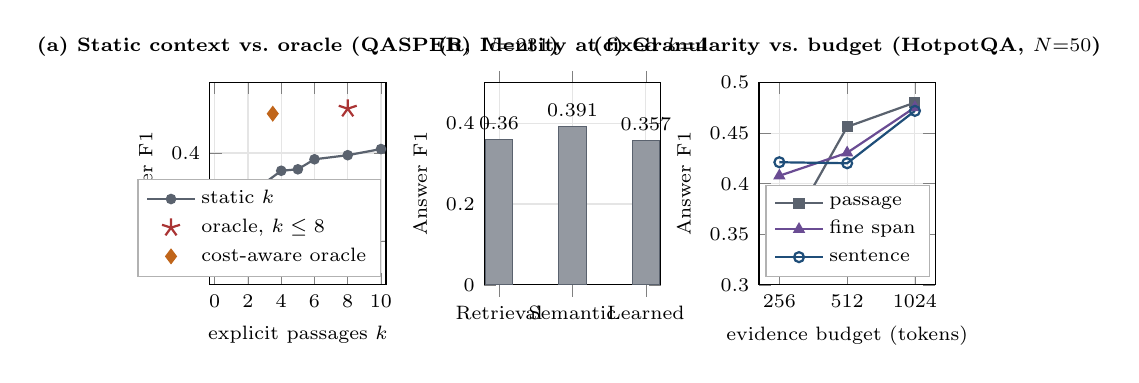
\begin{tikzpicture}
\begin{groupplot}[group style={group size=3 by 1,horizontal sep=1.25cm},width=0.315\textwidth,height=4.15cm,
  tick label style={font=\scriptsize},label style={font=\scriptsize},title style={font=\scriptsize\bfseries},grid=major,grid style={black!10}]
\nextgroupplot[title={(a) Static context vs.\ oracle (\qasper, $N{=}231$)},xlabel={explicit passages $k$},ylabel={Answer F1},xmin=-0.3,xmax=10.3,ymin=0.1,ymax=0.56,xtick={0,2,4,6,8,10},
  legend style={font=\scriptsize,at={(0.97,0.04)},anchor=south east,draw=black!30},legend cell align=left]
\addplot[cgray,thick,mark=*,mark size=1.5pt] coordinates {(0,.1388)(2,.3038)(4,.3596)(5,.3629)(6,.3857)(8,.3950)(10,.4090)};\addlegendentry{static $k$}
\addplot[only marks,mark=star,mark size=3.4pt,cred,thick] coordinates {(8,.5008)};\addlegendentry{oracle, $k\le8$}
\addplot[only marks,mark=diamond*,mark size=2.6pt,corange] coordinates {(3.49,.4894)};\addlegendentry{cost-aware oracle}
\nextgroupplot[title={(b) Identity at fixed $k{=}4$},ylabel={Answer F1},ybar,bar width=10pt,symbolic x coords={Retrieval,Semantic,Learned},xtick=data,ymin=0,ymax=0.5,
  nodes near coords,nodes near coords style={font=\scriptsize,/pgf/number format/fixed,/pgf/number format/precision=3}]
\addplot[fill=cgray!65,draw=cgray] coordinates {(Retrieval,.3596)(Semantic,.3913)(Learned,.3572)};
\nextgroupplot[title={(c) Granularity vs.\ budget (\hotpot, $N{=}50$)},xlabel={evidence budget (tokens)},ylabel={Answer F1},symbolic x coords={256,512,1024},xtick=data,ymin=0.30,ymax=0.50,enlarge x limits=0.15,
  legend style={font=\scriptsize,at={(0.97,0.04)},anchor=south east,draw=black!30},legend cell align=left]
\addplot[cgray,thick,mark=square*,mark size=1.6pt] coordinates {(256,.3375)(512,.4563)(1024,.4803)};\addlegendentry{passage}
\addplot[cpurple,thick,mark=triangle*,mark size=1.8pt] coordinates {(256,.4079)(512,.4306)(1024,.4755)};\addlegendentry{fine span}
\addplot[cblue,thick,mark=o,mark size=1.8pt] coordinates {(256,.4213)(512,.4203)(1024,.4721)};\addlegendentry{sentence}
\end{groupplot}
\end{tikzpicture}
\caption{Evidence behind the three pivots. (a) Outcome-selected oracles lie far above any static $k$ but cannot be deployed. (b) Selecting different passages at the same $k$ changes F1. (c) Sentences lead at 256 tokens and passages catch up at larger budgets; interaction intervals crossed zero, so the pattern is descriptive. Tiers differ between panels (Table~\ref{tab:tiers}).}\label{fig:early}
\end{figure*}

%=====================================================================
\section{QBGF: Query-Conditioned Budgeted Granularity Fusion}\label{sec:qbgf}
\paragraph{Motivation and intuition.} Sentences pack tightly but lose discourse; whole passages keep context but are expensive, and which is better varies by source and budget. For each retrieved passage, QBGF decides whether to \emph{discard it, keep its few most query-relevant sentences, or keep it whole}, and makes all these choices jointly so that the total fits the token budget.

\paragraph{Inputs and outputs.} Input: the query, the ten retrieved passages and the budget $B$. Output: a source-ordered evidence string of at most $B$ tokens for the frozen reader. Nothing is generated: every option is an extractive view of a retrieved source (Fig.~\ref{fig:qbgf}).

\begin{figure*}[t]\centering
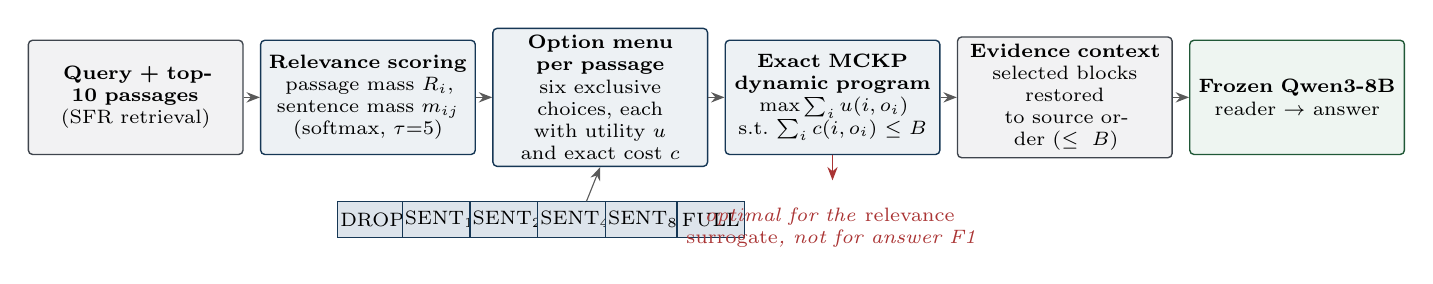
\begin{tikzpicture}[font=\scriptsize]
\foreach \n/\x/\c/\t in {1/0/cgray/{\textbf{Query + top-10 passages}\\(SFR retrieval)},
  2/2.95/cblue/{\textbf{Relevance scoring}\\passage mass $R_i$,\\sentence mass $m_{ij}$ (softmax, $\tau{=}5$)},
  3/5.9/cblue/{\textbf{Option menu per passage}\\six exclusive choices, each\\with utility $u$ and exact cost $c$},
  4/8.85/cblue/{\textbf{Exact MCKP dynamic program}\\$\max\sum_i u(i,o_i)$\\s.t.\ $\sum_i c(i,o_i)\le B$},
  5/11.8/cgray/{\textbf{Evidence context}\\selected blocks restored\\to source order ($\le B$)},
  6/14.75/cgreen/{\textbf{Frozen Qwen3-8B}\\reader $\to$ answer}}{
 \node[box=\c,text width=2.55cm,minimum height=1.45cm] (n\n) at (\x+1.275,0) {\t};}
\foreach \a/\b in {1/2,2/3,3/4,4/5,5/6}{\draw[arr](n\a.east)--(n\b.west);}
\foreach \i/\t in {0/DROP,1/{SENT$_{1}$},2/{SENT$_{2}$},3/{SENT$_{4}$},4/{SENT$_{8}$},5/FULL}{
 \node[draw=cblue!70!black,fill=cblue!15,minimum width=0.86cm,minimum height=0.45cm,inner sep=1pt,font=\scriptsize] at (3.85+0.86*\i+0.43,-1.55) {\t};}
\draw[arr,line width=0.4pt] (7.0,-1.32)--(n3.south);
\node[font=\scriptsize\itshape,text=cred,text width=4.0cm,align=center] at (10.1,-1.65) {optimal for the \emph{relevance surrogate}, not for answer F1};
\draw[arr,cred,line width=0.4pt] (n4.south)--++(0,-0.32);
\end{tikzpicture}
\caption{QBGF pipeline. Each passage is offered DROP, its top 1/2/4/8 query-similar sentences, or the full passage; the dynamic program picks one option per passage so the serialized evidence fits $B$. It uses no downstream-utility signal and generates no new text.}\label{fig:qbgf}
\end{figure*}

\paragraph{Formulation.} Let $s(p_i)$ and $s(s_{ij})$ be SFR cosine similarities of passage $i$ and of its sentence $j$ to the query. Passage and within-passage relevance masses are softmax-normalized ($\tau{=}5$):
\begin{align}
R_i&=\frac{e^{\tau s(p_i)}}{\sum_{m=1}^{K}e^{\tau s(p_m)}},\nonumber\\
m_{ij}&=\frac{e^{\tau s(s_{ij})}}{\sum_{\ell}e^{\tau s(s_{i\ell})}},\label{eq:mass}\\
u(i,\mathrm{SENT}_k)&=R_i\sum_{j\in\mathrm{top}\text{-}k}m_{ij},\nonumber\\
u(i,\mathrm{FULL})&=R_i,\quad u(i,\mathrm{DROP})=0.\nonumber
\end{align}
The cost $c(i,o)$ is the exact Qwen token length of the serialized block for option $o\in\mathcal O_i=\{\mathrm{DROP},\mathrm{SENT}_{1,2,4,8},\mathrm{FULL}\}$. QBGF solves the multiple-choice knapsack (MCKP)
\begin{equation}
\max_{o_i\in\mathcal O_i}\ \sum_{i=1}^{K}u(i,o_i)\quad\text{s.t.}\quad\sum_{i=1}^{K}c(i,o_i)\le B,\label{eq:mckp}
\end{equation}
exactly by dynamic programming over (passage, remaining budget) (Appendix~\ref{app:alg}). Blocks are tokenized separately with their trailing separator, so costs add exactly.

\paragraph{What QBGF optimizes, and what it does not.} The DP is globally optimal for the additive relevance surrogate~\eqref{eq:mckp}; it is \emph{not} optimal for answer F1 and has no stopping rule beyond feasibility. \textbf{Variants and comparators} (same pool, budgets and reader): \emph{no evidence}; \emph{passage} (retrieval-order whole passages); \emph{sentence} (global greedy ranking of sentences by query cosine; the baseline that is later locked); \emph{hybrid} (first three passages as sentences, the rest as finer spans); \emph{no-query} (uniform masses; upstream retrieval stays query-dependent); \emph{passage-only} (DROP/FULL) and \emph{sentence-only} (no FULL).

\subsection{Validation: ablation versus best comparator}
Table~\ref{tab:val} reports full validation ($N{=}8{,}337$). No method dominates: sentence selection leads \qasper-256 (0.2634) and \scifact-256 (0.7001); whole passages lead \scifact-1024 (0.6990); passage-only QBGF leads \hotpot-1024 (0.4525); the hybrid leads \hotpot-256 and \qasper-1024. \textbf{Against its own ablations} (Table~\ref{tab:abl}), query conditioning improves all six cells ($+0.020$ to $+0.187$ F1), reported significant in the registered Holm-adjusted family ($p_{\mathrm{Holm}}\le0.0114$). \textbf{Against the best comparator} the picture differs: removing FULL changes QBGF by at most $\pm0.0001$ F1 at 256 tokens, and at 1,024 sentence-only beats full QBGF on \scifact ($+0.024$) and passage-only on \hotpot ($+0.020$). Query conditioning helps; mixed-granularity fusion is not shown to be necessary.

\begin{table*}[t]\centering\SmallTable
\caption{Full validation ($N{=}8{,}337$). \hotpot/\qasper: Answer F1; \scifact: macro-F1; bold = best point estimate per row (rows are different tasks and budgets).}\label{tab:val}
\begin{tabular}{llrrrrrrrr}\toprule
Dataset & $B$ & None & Passage & Sentence & Hybrid & QBGF & No-query & Passage-only & Sentence-only\\\midrule
\hotpot & 256 & .1653 & .4070 & .4082 & \textbf{.4253} & .4121 & .3086 & .3935 & .4122\\
\hotpot & 1024 & .1653 & .4521 & .4233 & .4364 & .4323 & .4123 & \textbf{.4525} & .4323\\
\qasper & 256 & .0822 & .1693 & \textbf{.2634} & .2544 & .2355 & .1473 & .1693 & .2356\\
\qasper & 1024 & .0822 & .2880 & .2988 & \textbf{.2995} & .2951 & .2284 & .2896 & .2977\\
\scifact & 256 & .4207 & .4564 & \textbf{.7001} & .6856 & .6750 & .4880 & .4578 & .6750\\
\scifact & 1024 & .4207 & \textbf{.6990} & .6704 & .6859 & .6604 & .5426 & .6031 & .6847\\\bottomrule
\end{tabular}\end{table*}

\paragraph{Locked selection and confirmation.} \qbgf would replace the sentence baseline only if it were noninferior in \emph{all six} cells (margin 0.003 F1 for QA, 0.010 macro-F1 for \scifact; paired 10,000-resample cluster bootstrap, seed 42) and used no more mean prompt tokens in any cell. Only \hotpot-1024 cleared the margin ($+0.0090$, 95\% CI $[+0.0045,+0.0135]$); \qasper-256 was $-0.0279$ $[-0.0410,-0.0149]$ and four cells were inconclusive (Appendix~\ref{app:stats}). QBGF used 2.5--8.2 fewer prompt tokens, so it failed on quality, not cost; the sentence baseline was locked \emph{before} confirmation was opened. On the reserved cohort (Table~\ref{tab:conf}) the locked policy beats no evidence in all four cells; on \scifact-256 it reaches 0.7014 versus 0.4138 for passages ($+0.2876$, $p_{\mathrm{Holm}}{=}0.0356$), while passages are competitive again at 1,024 (0.7680 vs.\ 0.7440, interval crossing zero). QBGF beats the sentence policy on \hotpot-1024 ($+0.0344$, $p_{\mathrm{Holm}}{=}0.0316$, secondary family), which neither overturns the lock nor identifies which QBGF component helps. No universal granularity winner emerges.

\begin{table}[t]\centering\SmallTable
\caption{Ablation: full QBGF minus restricted variant (from Table~\ref{tab:val}); positive favors full QBGF. Descriptive differences, not extra tests.}\label{tab:abl}
\begin{tabular}{llrrr}\toprule
Task & $B$ & $-$No-query & $-$Passage-only & $-$Sent.-only\\\midrule
\hotpot & 256 & +.1035 & +.0186 & $-.0001$\\
\hotpot & 1024 & +.0200 & $-.0202$ & .0000\\
\qasper & 256 & +.0882 & +.0662 & $-.0001$\\
\qasper & 1024 & +.0667 & +.0055 & $-.0026$\\
\scifact & 256 & +.1870 & +.2172 & .0000\\
\scifact & 1024 & +.1178 & +.0573 & $-.0243$\\\bottomrule
\end{tabular}\end{table}

\begin{table}[t]\centering\SmallTable
\caption{Reserved confirmation (\hotpot $N{=}200$; \scifact $N{=}50$). $\dagger$ = locked policy.}\label{tab:conf}
\begin{tabular}{llrrrrr}\toprule
Task & $B$ & None & Passage & Sent.$^\dagger$ & Hybrid & QBGF\\\midrule
\hotpot & 256 & .1399 & .4227 & .4373 & \textbf{.4622} & .4406\\
\hotpot & 1024 & .1399 & .4589 & .4329 & .4570 & \textbf{.4672}\\
\scifact & 256 & .3686 & .4138 & .7014 & \textbf{.7067} & .6870\\
\scifact & 1024 & .3686 & \textbf{.7680} & .7440 & .7168 & .6346\\\bottomrule
\end{tabular}\end{table}

%=====================================================================
\section{Relevance Is Not Utility: Leave-One-Out Diagnosis}\label{sec:loo}
\paragraph{Why LOO.} A solver that is exact for relevance can still select evidence that barely changes the answer. We measure this directly (Fig.~\ref{fig:loo}a): take the selected context $E$, remove one unit $u_i$, keep all other units unchanged, \emph{do not refill} the freed tokens, and regenerate with the frozen reader:
\begin{equation}
\Delta_i=\mathrm{Score}(E\setminus\{u_i\})-\mathrm{Score}(E).\label{eq:loo}
\end{equation}
\textbf{Sign convention.} A \emph{negative} $\Delta_i$ means removal made the answer worse, i.e.\ the unit was \emph{helpful}. For QA, Score is per-query Answer F1 and we call a unit helpful if $\Delta_i<-\delta$, harmful if $\Delta_i>+\delta$ and neutral otherwise ($\delta{=}0.01$); for \scifact Score is per-claim correctness and $\delta{=}0$. Neutral means no detectable \emph{single-deletion} effect in this context, not irrelevance. The classifier labels of \S\ref{sec:bea} use the strict sign ($\delta{=}0$).

\begin{figure*}[t]\centering
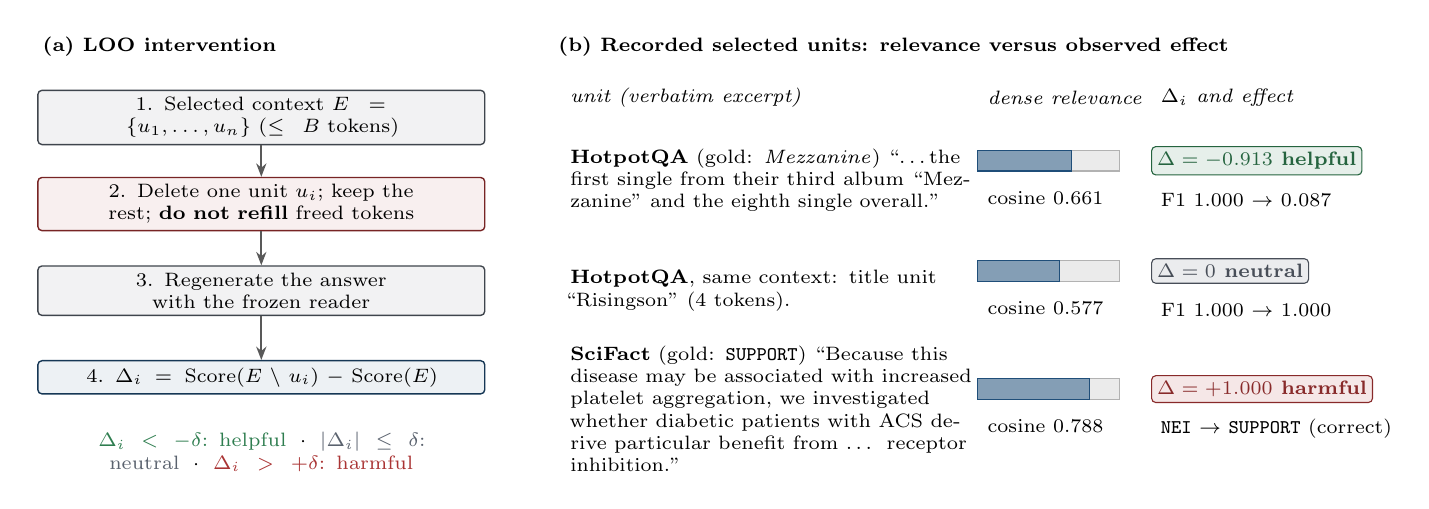
\begin{tikzpicture}[font=\scriptsize]
% panel (a): procedure
\node[font=\scriptsize\bfseries,anchor=west] at (0,0.55) {(a) LOO intervention};
\node[box=cgray,text width=5.5cm] (a1) at (2.9,-0.35) {1. Selected context $E=\{u_1,\dots,u_n\}$ ($\le B$ tokens)};
\node[box=cred,text width=5.5cm] (a2) at (2.9,-1.45) {2. Delete one unit $u_i$; keep the rest; \textbf{do not refill} freed tokens};
\node[box=cgray,text width=5.5cm] (a3) at (2.9,-2.55) {3. Regenerate the answer with the frozen reader};
\node[box=cblue,text width=5.5cm] (a4) at (2.9,-3.65) {4. $\Delta_i=\mathrm{Score}(E\setminus u_i)-\mathrm{Score}(E)$};
\draw[arr](a1)--(a2);\draw[arr](a2)--(a3);\draw[arr](a3)--(a4);
\node[font=\scriptsize,text width=5.7cm,align=center] at (2.9,-4.6) {\textcolor{cgreen}{$\Delta_i<-\delta$: helpful}\; $\cdot$\; \textcolor{cgray}{$|\Delta_i|\le\delta$: neutral}\; $\cdot$\; \textcolor{cred}{$\Delta_i>+\delta$: harmful}};
% panel (b): examples
\node[font=\scriptsize\bfseries,anchor=west] at (6.55,0.55) {(b) Recorded selected units: relevance versus observed effect};
\node[font=\scriptsize\itshape,anchor=west] at (6.7,-0.1) {unit (verbatim excerpt)};
\node[font=\scriptsize\itshape,anchor=west] at (12.0,-0.1) {dense relevance};
\node[font=\scriptsize\itshape,anchor=west] at (14.2,-0.1) {$\Delta_i$ and effect};
\foreach \y/\txt/\rel/\col/\lab/\sub in {
 -1.15/{\textbf{\hotpot} (gold: \emph{Mezzanine}) ``\ldots the first single from their third album ``Mezzanine'' and the eighth single overall.''}/0.661/cgreen/{$\Delta=-0.913$ helpful}/{F1 1.000 $\to$ 0.087},
 -2.55/{\textbf{\hotpot}, same context: title unit ``Risingson'' (4 tokens).}/0.577/cgray/{$\Delta=0$ neutral}/{F1 1.000 $\to$ 1.000},
 -4.05/{\textbf{\scifact} (gold: \texttt{SUPPORT}) ``Because this disease may be associated with increased platelet aggregation, we investigated whether diabetic patients with ACS derive particular benefit from \ldots{} receptor inhibition.''}/0.788/cred/{$\Delta=+1.000$ harmful}/{\texttt{NEI} $\to$ \texttt{SUPPORT} (correct)}}{
 \node[anchor=west,text width=5.1cm,align=left,font=\scriptsize] at (6.7,\y) {\txt};
 \draw[fill=black!8,draw=black!30] (12.0,\y+0.12) rectangle ++(1.8,0.26);
 \draw[fill=cblue!55,draw=cblue] (12.0,\y+0.12) rectangle ++(1.8*\rel,0.26);
 \node[anchor=west,font=\scriptsize] at (12.0,\y-0.22) {cosine \rel};
 \node[draw=\col!80!black,fill=\col!12,rounded corners=1.5pt,inner sep=2pt,anchor=west,font=\scriptsize\bfseries,text=\col!80!black] at (14.2,\y+0.25) {\lab};
 \node[anchor=west,font=\scriptsize] at (14.2,\y-0.25) {\sub};}
\end{tikzpicture}
\caption{(a) The LOO intervention and its sign convention. (b) Three real interventions: relevance does not predict effect. The most relevant unit (0.788, parent rank 1) is the harmful one: in that context another selected sentence already states an increased bleeding risk, and deleting this trial sentence flips the output from \texttt{NOT\_ENOUGH\_INFO} to the correct \texttt{SUPPORT}. This is a context-specific deletion effect, not intrinsic harmfulness or an identified internal mechanism.}\label{fig:loo}
\end{figure*}

\paragraph{Findings.} Most selected units are neutral (69.5--98.9\% in the representative conditions of Table~\ref{tab:loo}), and the Spearman correlation between dense relevance and deletion utility is at most 0.134 there. Across the 12 conditions of the project's attribution study (50 queries per dataset), bootstrap intervals for this correlation include zero in 10; the exceptions are \hotpot passage-only at 1,024 ($\rho{=}0.221$) and \scifact QBGF at 256 ($\rho{=}0.134$) (Appendix~\ref{app:stats}). Qualitative review of 16 query profiles suggested recurring patterns: high-similarity distractors, redundant entity relations and sentence fragmentation that removes antecedents. These are plausible mechanisms, not identified causes.

\paragraph{Caveats.} LOO is state-dependent: in multi-hop questions two complementary facts can each look neutral when the partner is missing, so neutral units are not necessarily dispensable. LOO motivates learning a utility signal; it does not identify universal causal importance.

\begin{table}[t]\centering\SmallTable
\caption{Representative LOO distributions on the 50-query-per-dataset attribution cohort. H/Q/S = \hotpot/\qasper/\scifact; $\rho$ = Spearman correlation of dense relevance with deletion utility. Fractions count selected-unit interventions.}\label{tab:loo}
\begin{tabular}{llrrrr}\toprule
Task & Policy / $B$ & $\rho$ & Helpful & Neutral & Harmful\\\midrule
H & QBGF / 256 & .068 & 8.9\% & 84.0\% & 7.2\%\\
H & QBGF / 1024 & .010 & 5.0\% & 88.1\% & 6.9\%\\
Q & Sentence / 256 & .126 & 15.6\% & 76.4\% & 7.9\%\\
Q & QBGF / 256 & .104 & 17.0\% & 69.5\% & 13.5\%\\
S & QBGF / 256 & .134 & 2.8\% & 92.2\% & 4.9\%\\
S & QBGF / 1024 & .044 & 0.5\% & 98.9\% & 0.6\%\\\bottomrule
\end{tabular}\end{table}

%=====================================================================
\section{BEA: Incremental and Utility-Aware Allocation}\label{sec:bea}
QBGF scores options largely independently of what else is selected and fills the budget whenever a positive-utility option fits. BEA starts instead from an empty context, repeatedly accepts the next transition with the highest estimated gain \emph{per added token}, recomputes gains after every acceptance, and stops when the best remaining gain is too small, leaving budget unused. No reader call occurs during selection, and BEA builds no document tree. Figure~\ref{fig:cmp} contrasts the three allocators.

\begin{figure*}[t]\centering
\newcounter{pnlcnt}
\newcommand{\panel}[8]{% #1 x, #2 colour, #3 title, #4..#7 node texts, #8 footer
 \stepcounter{pnlcnt}%
 \node[fill=#2,text=white,font=\scriptsize\bfseries,minimum width=5.65cm,minimum height=0.46cm,anchor=north west,inner sep=2pt] (h\thepnlcnt) at (#1,0) {#3};
 \node[box=#2,text width=5.3cm,minimum height=0.78cm,anchor=north] (p\thepnlcnt a) at ($(h\thepnlcnt.south)+(0,-0.22)$) {#4};
 \node[box=#2,text width=5.3cm,minimum height=0.78cm,anchor=north] (p\thepnlcnt b) at ($(p\thepnlcnt a.south)+(0,-0.26)$) {#5};
 \node[box=#2,text width=5.3cm,minimum height=0.78cm,anchor=north] (p\thepnlcnt c) at ($(p\thepnlcnt b.south)+(0,-0.26)$) {#6};
 \node[box=#2,text width=5.3cm,minimum height=0.78cm,anchor=north] (p\thepnlcnt d) at ($(p\thepnlcnt c.south)+(0,-0.26)$) {#7};
 \draw[arr](p\thepnlcnt a)--(p\thepnlcnt b);\draw[arr](p\thepnlcnt b)--(p\thepnlcnt c);\draw[arr](p\thepnlcnt c)--(p\thepnlcnt d);
 \node[draw=#2,fill=#2!15,rounded corners=1.5pt,text width=5.3cm,align=center,font=\scriptsize\bfseries,inner sep=2pt,anchor=north] at ($(p\thepnlcnt d.south)+(0,-0.22)$) {#8};}
\begin{tikzpicture}
\setcounter{pnlcnt}{0}%
\panel{0}{cblue}{\qbgf: global packing, one shot}{score all 10 passages once: $R_i$, $m_{ij}$}{choose \emph{one of six options} per passage: DROP / SENT$_{1,2,4,8}$ / FULL}{maximize $\sum u$ (relevance mass) s.t.\ $\sum c\le B$: exact DP}{output once; stops only when feasibility binds}{optimizes relevance; no utility signal}
\panel{6.05}{corange}{\vone: incremental, heuristic}{start from an \emph{empty} context}{score each next addition: $g=r+0.5\,\Delta C-0.5\,\mathrm{Red}$; density $d=g/\Delta c$}{add the best if $d\ge0.01$ (FULL also needs gate 0.05); recompute all scores}{otherwise stop; budget may stay unused (starvation risk)}{adds coverage, redundancy and stopping}
\panel{12.1}{cgreen}{\vtwo: incremental, learned}{start from an \emph{empty} context}{score: $U=\Phelp\cdot\max(0,g)$, $D=U/\Delta c$; $\Phelp$ from a LOO-trained classifier}{add the best if $D\ge8{\times}10^{-5}$; targets 1/2/4/8 sentences or FULL; recompute}{otherwise stop; threshold calibration unresolved}{adds a learned helpfulness weight}
\end{tikzpicture}
\caption{The three allocators side by side. \qbgf chooses a fidelity per passage jointly and once; \vone grows the context one transition at a time with a heuristic marginal value and an early-stopping rule; \vtwo keeps that loop but multiplies the gain by a classifier's estimate of how likely such evidence was to help in past LOO experiments.}\label{fig:cmp}
\end{figure*}

\begin{table*}[t]\centering\SmallTable
\caption{Exploratory matched development comparison (50 queries per dataset; \emph{not} a confirmation experiment). \hotpot/\qasper: Answer F1; \scifact: macro-F1; bold = best point estimate per row.}\label{tab:bea}
\begin{tabular}{llrrrrr}\toprule
Dataset & $B$ & Sentence & \qbgf & \vone & \vtwo & MiniLM cross-encoder\\\midrule
\hotpot & 256 & .3661 & .4042 & .2976 & \textbf{.4352} & .3404\\
\hotpot & 1024 & .3893 & .4020 & .3441 & \textbf{.4234} & .3618\\
\qasper & 256 & \textbf{.2668} & .2641 & .1868 & .2618 & .2641\\
\qasper & 1024 & .2896 & \textbf{.2964} & .2084 & .2904 & .2827\\
\scifact & 256 & .6289 & .5310 & .6127 & .5522 & \textbf{.6855}\\
\scifact & 1024 & .5533 & .5881 & .6432 & .5772 & \textbf{.6479}\\\bottomrule
\end{tabular}\end{table*}

\subsection{BEA-V1: heuristic marginal value and its failure}
\paragraph{Intuition and procedure.} Add a sentence if it is relevant, covers part of the question not yet covered, and does not repeat what is already selected; prefer cheap additions; after two accepted sentences from one source, a FULL upgrade of that source may also compete. Query aspects $A(q)$ are at most six deterministic lexical clauses of the query (split on question marks, commas, semicolons and conjunctions). For the selected set $S$, with normalized SFR vectors $v_i$, $v_a$ and query vector $e_q$:
\begin{align}
r_i&=\cos(e_q,v_i),\nonumber\\
h_a(S)&=\max\!\left(0,\max_{j\in S}\cos(v_a,v_j)\right),\nonumber\\
\Delta C_i(S)&=\sum_{a\in A(q)}\max\bigl(0,\cos(v_a,v_i)-h_a(S)\bigr),\nonumber\\
\mathrm{Red}_i(S)&=\max_{j\in S}\cos(v_i,v_j),\nonumber\\
g_i(S)&=r_i+0.5\Delta C_i(S)-0.5\mathrm{Red}_i(S),\nonumber\\
d_i&=\frac{g_i(S)}{\Delta c_i}.\label{eq:v1}
\end{align}
$\Delta c$ is the change in serialized token cost; non-positive costs get priority. V1 accepts the highest-density admissible transition if $d\ge0.01$ (FULL upgrades also need a local gate of $0.05$), otherwise it stops. The thresholds come from an allocation-only calibration on nine development queries. Worked example: for the 56-token Goya sentence at a later state, relevance $0.806$, new coverage $0.096$ and redundancy $0.758$ give $g=0.475$ and $d=0.00848<0.01$: it is rejected although it is the decisive bridge.

\begin{case}[title={Context starvation (\qasper, $B{=}1024$)}]{corange}
\emph{Question:} ``What are the five different binary classification tasks?'' \vone made 15 additions, stopped after \textbf{245} tokens (779 unused) with last marginal density $0.009965<0.01$, and its context held stimulus words instead of the task list: F1 $=0$. Sentence and \qbgf used 1,022 and 1,018 tokens, exposed the list and scored 0.7826 (\vtwo: 965 tokens, 0.7826). On matched \hotpot-1024, \vone used 284 tokens on average and scored 0.3441 versus 0.3893 for sentences. An early-stopping rule can reject evidence that is individually low-scoring but necessary; we do not claim one threshold decision causes every error.
\end{case}

\subsection{BEA-V2: weight gains by learned helpfulness}
\paragraph{What changes.} \vtwo keeps V1's relevance, coverage, redundancy and cost definitions but multiplies the non-negative gain by a classifier's estimate of how likely such evidence was to help the reader in past LOO experiments.

\paragraph{Labels and predictor.} Historical LOO exports give 8,537 sentence observations (555 helpful, 552 harmful, 7,430 neutral; repeated across methods and budgets). The label uses the strict sign of~\eqref{eq:loo}: $y^{\mathrm{help}}_i=\mathbb 1[\Delta_i<0]$. Per dataset, an L2 logistic regression (standardized features, $C{=}1$, no class weights) on 12 \emph{pre-generation} features (query--sentence and passage cosines, retrieval and within-passage ranks, position, token costs, sentence count, budget, pool width, pool-similarity statistics) estimates $\Phelp(i)=\sigma(w^\top x_i+b)$. Five-fold GroupKFold splits by query (\hotpot), paper (\qasper) or cited-document component (\scifact); each evaluation query uses its held-out-fold model. The value and density of a transition $a$ are
\begin{equation}
U_t(a)=\sum_{i\in a}\Phelp(i)\max\bigl(0,g_i(S_{t,i})\bigr),\qquad D_t(a)=\frac{U_t(a)}{\Delta c_t(a)},\label{eq:v2}
\end{equation}
where $S_{t,i}$ is the hypothetical state updated within a compound action. \textbf{At inference} no gold answer, LOO intervention or reader feedback is used; $\Phelp$ is computed from pre-generation features only, the budget is enforced on serialized token cost, and the harmfulness label is diagnostic only. \vtwo targets 1/2/4/8 sentences per source, allows FULL after two positive contributions, drops V1's local 0.05 gate, and stops when $D<\tau{=}8{\times}10^{-5}$ (an exploratory operating point), when no positive feasible candidate remains, or when the budget is full.

\paragraph{How good is the predictor?} Pooled out-of-fold ROC-AUC is 0.625/0.590/0.836 and average precision 0.106/0.202/0.072 for \hotpot/\qasper/\scifact (positive prevalence 0.064/0.094/0.017): some ranking signal, limited discrimination, and no claim of calibrated probabilities or of fresh-context addition utility (Appendix~\ref{app:alg}). \textbf{Worked example.} At step 1 on the Goya bridge sentence, \vtwo recorded relevance $0.806$, coverage $0.803$, redundancy $0$, $\Phelp{=}0.126$, hence $g{=}1.208$, $U{=}0.152$, $D{=}0.00272$; it was selected first and the answer \emph{Invader (Invasor)} (F1 $1$) was recovered (the V1 and V2 scores refer to different states and are not a controlled comparison).

\subsection{Matched exploratory comparison}
Table~\ref{tab:bea} (with a supplemental graphical comparison in Fig.~\ref{fig:res}) compares all methods on the same 50 queries per dataset at both budgets after the policy had been locked. At $\tau{=}8{\times}10^{-5}$, \vtwo has the highest \hotpot F1 at both budgets (0.4352 vs.\ 0.3661 for sentences, $+0.0691$; 0.4234 vs.\ 0.3893, $+0.0341$) and exceeds \qbgf (0.4042, 0.4020). Elsewhere other methods lead: sentences on \qasper-256 (0.2668), \qbgf on \qasper-1024 (0.2964), and the MiniLM cross-encoder on \scifact (0.6855, 0.6479); \vtwo is within 0.005 F1 of sentences on \qasper, below them on \scifact-256 (0.5522 vs.\ 0.6289) and above them at 1,024 (0.5772 vs.\ 0.5533). \vone is lowest on \hotpot and \qasper.





\paragraph{Boundaries of these results.} (i) The 50 queries per dataset are development data that overlap validation. (ii) The threshold $\tau$ was examined after an allocation-only calibration on nine queries failed its pre-specified utilization and coverage gates. (iii) A 24-test Holm family comparing MiniLM with four controls found no significant comparison ($p_{\mathrm{Holm}}\ge0.2592$) and does \emph{not} test \vtwo against sentences. (iv) V1$\to$V2 changes gates and transitions as well as adding the predictor, and no \vtwo run with $\Phelp\equiv1$ exists, so the predictor's contribution is not isolated. (v) The classifier has no independent confirmation. The results are promising but do not overturn the locked sentence policy.

%=====================================================================
\section{Discussion and Limitations}\label{sec:disc}
\textbf{What the evidence supports.} (1)~Context demand is heterogeneous, but a scalar $k$ is hard to predict because false stops cost far more than false expansions. (2)~Which sources survive and in which representation both matter at fixed $k$; reader-interface differences can confound comparisons. (3)~Sentence units are a strong compact baseline under tight budgets, while whole passages are competitive at larger budgets (descriptive). (4)~Query conditioning contributes to QBGF, yet exact optimization of a relevance surrogate does not guarantee downstream quality. (5)~LOO outcomes motivate learned utility, which helps in exploratory multi-hop runs but remains an imperfect proxy for the value of a \emph{new} addition. One reason the sentence baseline may be competitive is that it combines a query-relevance signal with compact evidence units without a learned stopping rule that could amplify prediction error.

\textbf{Limitations.} \hotpot uses its distractor pool, not open-domain retrieval. Final results use one reader (base Qwen3-8B, FP16), chosen partly because it obeyed the \scifact label interface; the SARA projector and LoRA are Mistral-specific, so the study is not a cross-family test of latent compression. The granularity pilot has 50 queries; formal interaction intervals did not establish a universal effect. LOO measures single deletions from one frozen context and cannot capture complementary evidence. \qasper is excluded from confirmation because earlier exploratory runs exposed its test-query IDs. We measured no matched end-to-end latency or memory, so we make no serving-efficiency claim; repeated LOO generations and classifier fitting are research costs, not free inference. \textbf{Future work:} larger, stratified threshold calibration; a $\Phelp\equiv1$ ablation; interaction-aware attribution (pair deletion); and a systems evaluation of allocator overhead.

%=====================================================================
\section{Conclusion}\label{sec:concl}
We began with a SARA-inspired question, how much readable evidence each query needs, and found headroom that learned controllers could not capture. The investigation then moved from \emph{quantity} to \emph{identity} and \emph{granularity}, and to QBGF, an exact fidelity allocator whose query conditioning helps but which does not reliably beat a locked sentence baseline. LOO interventions identified the deeper problem: relevance is only weakly aligned with a unit's effect on the reader. BEA-V1 showed that early stopping can starve the context; BEA-V2, which weights gains by learned helpfulness, leads \hotpot at both budgets in exploratory matched runs but is mixed on \qasper and \scifact and unconfirmed. Budget-aware selection, query conditioning and representation granularity matter; optimizing semantic relevance alone does not reliably optimize answer quality. \textbf{A validated, transferable estimate of downstream evidence utility, together with a calibrated stopping rule, is a more promising next target than a more elaborate packer.}

%=====================================================================
\clearpage
\onecolumn
%================== REFERENCES AND APPENDIX START HERE ==================
\begin{thebibliography}{99}\small
\bibitem{lewis2020rag} P.~Lewis, E.~Perez, A.~Piktus, F.~Petroni, V.~Karpukhin, N.~Goyal, H.~K\"{u}ttler, M.~Lewis, W.~Yih, T.~Rockt\"{a}schel, S.~Riedel, D.~Kiela. Retrieval-augmented generation for knowledge-intensive NLP tasks. \emph{NeurIPS}, 2020.
\bibitem{jin2026sara} Y.~Jin, K.~Sharma, V.~Rakesh, Y.~Dou, M.~Pan, M.~Das, S.~Kumar. SARA: Selective and adaptive retrieval-augmented generation with context compression. \emph{ACL}, 2026.
\bibitem{recomp2024} F.~Xu, W.~Shi, E.~Choi. RECOMP: Improving retrieval-augmented LMs with compression and selective augmentation. \emph{ICLR}, 2024.
\bibitem{liu2024lost} N.~F. Liu, K.~Lin, J.~Hewitt, A.~Paranjape, M.~Bevilacqua, F.~Petroni, P.~Liang. Lost in the middle: How language models use long contexts. \emph{TACL} 12:157--173, 2024.
\bibitem{yang2018hotpotqa} Z.~Yang, P.~Qi, S.~Zhang, Y.~Bengio, W.~W. Cohen, R.~Salakhutdinov, C.~D. Manning. HotpotQA: A dataset for diverse, explainable multi-hop question answering. \emph{EMNLP}, 2018.
\bibitem{dasigi2021qasper} P.~Dasigi, K.~Lo, I.~Beltagy, A.~Cohan, N.~A. Smith, M.~Gardner. A dataset of information-seeking questions and answers anchored in research papers. \emph{NAACL}, 2021.
\bibitem{wadden2020scifact} D.~Wadden, S.~Lin, K.~Lo, L.~L. Wang, M.~van Zuylen, A.~Cohan, H.~Hajishirzi. Fact or fiction: Verifying scientific claims. \emph{EMNLP}, 2020.
\bibitem{chen2024densex} T.~Chen, H.~Wang, S.~Chen, W.~Yu, K.~Ma, X.~Zhao, H.~Zhang, D.~Yu. Dense X Retrieval: What retrieval granularity should we use? \emph{EMNLP}, 2024.
\bibitem{pan2024llmlingua2} Z.~Pan, Q.~Wu, H.~Jiang, M.~Xia, X.~Luo, J.~Zhang, Q.~Lin, V.~R\"uhle, Y.~Yang, C.-Y. Lin, H.~V. Zhao, L.~Qiu, D.~Zhang. LLMLingua-2: Data distillation for efficient and faithful task-agnostic prompt compression. \emph{Findings of ACL}, 2024.
\bibitem{xu2026selfcorrecting} S.~Xu, Z.~Wu, X.~Jia, Y.~Wang, K.~Liu, A.~X. Dong. Self-Correcting RAG: Enhancing faithfulness via MMKP context selection and NLI-guided MCTS. arXiv:2604.10734, 2026.
\bibitem{jeong2024adaptive} S.~Jeong, J.~Baek, S.~Cho, S.~J. Hwang, J.~Park. Adaptive-RAG: Learning to adapt retrieval-augmented large language models through question complexity. \emph{NAACL}, 2024.
\bibitem{minilmreranker} Sentence Transformers. cross-encoder/ms-marco-MiniLM-L6-v2, model card. \url{https://huggingface.co/cross-encoder/ms-marco-MiniLM-L6-v2}. Accessed Nov.\ 2026.
\end{thebibliography}

%=====================================================================
\appendix
\setlength{\parskip}{2.3pt}
\setlength{\parindent}{0pt}
\captionsetup{font=small,skip=4pt}
\section{Algorithm Specifications and Predictor Details}\label{app:alg}
\subsection{QBGF: exact dynamic program}
\begin{apbox}[title={Algorithm A1: QBGF allocation (input: passages $p_{1..K}$, query, budget $B$)}]
\begin{enumerate}
\item Compute $R_i$ and $m_{ij}$ with $\tau{=}5$ (Eq.~\ref{eq:mass}); rank sentences within each passage by query cosine.
\item For each $i$ and option $o\in\{\mathrm{DROP},\mathrm{SENT}_{1,2,4,8},\mathrm{FULL}\}$: serialize the block (source-ordered sentences, trailing separator), tokenize with the Qwen tokenizer to get $c(i,o)$, and set $u(i,o)$ by Eq.~\ref{eq:mass}.
\item $V_0(b){=}0$ for $b{=}0..B$. For $i{=}1..K$: $V_i(b)=\max_{o:\,c(i,o)\le b}\{V_{i-1}(b-c(i,o))+u(i,o)\}$.
\item Backtrack from $V_K(B)$ to recover $o_i$. Ties within $10^{-12}$: prefer utility rounded to 12 decimals, then lower cost, then lexicographic option path.
\item Restore selected blocks and sentences to source order; concatenate the token-ID blocks and return.
\end{enumerate}
Complexity $O(6KB)$. Optimality holds for the finite additive surrogate; retokenizing the concatenated \emph{string} may give a different length, so the budget is defined on token-ID blocks.
\end{apbox}

\subsection{BEA-V1 and BEA-V2}
\begin{apbox}[title={Algorithm A2: BEA-V1 / BEA-V2 incremental allocation}]
\begin{enumerate}
\item $S{\leftarrow}\emptyset$; extract query aspects $A(q)$ (at most six clauses; fewer than two words dropped; duplicates removed; if none, use the whole query).
\item Enumerate eligible transitions: add an unselected sentence; or upgrade a source to FULL after two positive contributions. \textbf{V2} instead uses per-source sentence-count targets $1,2,4,8$ (capped by availability) plus FULL.
\item Score every transition under the current state: V1 $g_i$ (Eq.~\ref{eq:v1}); V2 $U_t=\sum_i\Phelp(i)\max(0,g_i(S_{t,i}))$ with the hypothetical state updated inside a compound action. FULL scans remaining parent sentences in source order and accumulates gains above the local gate ($0.05$ in V1; none in V2).
\item Density $d{=}g/\Delta c$ (V1) or $D{=}U/\Delta c$ (V2); $\Delta c{\le}0$ receives priority. Choose the highest density (ties: gain, incremental cost, source order, transition kind).
\item If the density is below the threshold ($0.01$ for V1; $8{\times}10^{-5}$ for V2), the gain is non-positive, or nothing fits: \textbf{stop} (V1 logs \texttt{LOW\_MARGINAL\_VALUE}). Otherwise apply the transition, recompute all scores, repeat.
\end{enumerate}
The V1 value $0.01$ overrides a retained default of $0.001$ (verified in the starvation run). A V2 allocation-only calibration over ten initial and four refined thresholds on nine development queries (both budgets) satisfied no setting for all pre-specified utilization and stopping constraints, so $8{\times}10^{-5}$ is exploratory.
\end{apbox}

\begin{table}[H]\centering\small\setlength{\tabcolsep}{5pt}
\caption{Pre-generation features of the helpfulness classifier (shared by training and inference; no imputation; standardized on training folds).}\label{tab:feat}
\begin{tabular}{rl}\toprule
No. & Feature\\\midrule
1--2 & query--sentence cosine; query--passage cosine\\
3--4 & retrieval rank of parent; within-parent relevance rank\\
5 & normalized source position of the sentence\\
6--7 & sentence token cost; parent passage token cost\\
8--10 & parent sentence count; budget (256/1024); pool width\\
11--12 & mean and maximum cosine to other candidate sentences\\\bottomrule
\end{tabular}\end{table}

\begin{table}[H]\centering\small\setlength{\tabcolsep}{5pt}
\caption{Out-of-fold diagnostics of the helpfulness classifier (probability cut-off 0.5 is descriptive; allocation uses the continuous probability). TN/FP/FN/TP in the last column.}\label{tab:cls}
\begin{tabular}{lrrrrl}\toprule
Task & Rows & Pos. & ROC-AUC & AP & Confusion\\\midrule
\hotpot & 2,941 & 188 & .6249 & .1064 & 2753/0/188/0\\
\qasper & 3,543 & 332 & .5897 & .2024 & 3204/7/317/15\\
\scifact & 2,053 & 35 & .8361 & .0721 & 2018/0/35/0\\\bottomrule
\end{tabular}\end{table}
An always-negative model would reach 93.5\% accuracy, so accuracy is uninformative; recall at 0.5 is near zero (0.000/0.045/0.000) although the continuous score still ranks candidates. Brier scores are .0593/.0828/.0167. Observations repeat across historical methods and budgets, come from development queries that overlap validation, and measure \emph{deletion} effects in selected contexts; grouped cross-fitting removes same-group leakage but supplies no independent confirmation or retraining uncertainty.

\section{Additional Experiments}\label{app:early}
\subsection{Visual summary of the matched exploratory comparison}
\begin{figure}[H]\centering
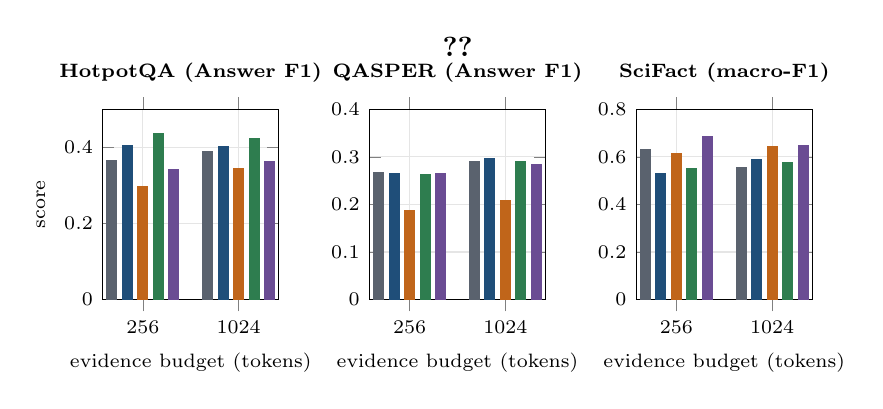
\begin{tikzpicture}
\begin{groupplot}[group style={group size=3 by 1,horizontal sep=1.15cm},ybar,/pgf/bar width=3.6pt,width=0.315\textwidth,height=4.0cm,symbolic x coords={256,1024},xtick=data,enlarge x limits=0.42,
  tick label style={font=\scriptsize},label style={font=\scriptsize},title style={font=\scriptsize\bfseries},xlabel={evidence budget (tokens)},grid=major,grid style={black!10}]
\nextgroupplot[title={\hotpot (Answer F1)},ymin=0,ymax=0.5,ylabel={score},legend to name=methleg,legend columns=5,legend style={font=\scriptsize,draw=black!30,/tikz/every even column/.append style={column sep=6pt}}]
\addplot[fill=cgray,draw=cgray] coordinates {(256,.3661)(1024,.3893)};\addlegendentry{Sentence}
\addplot[fill=cblue,draw=cblue] coordinates {(256,.4042)(1024,.4020)};\addlegendentry{QBGF}
\addplot[fill=corange,draw=corange] coordinates {(256,.2976)(1024,.3441)};\addlegendentry{BEA-V1}
\addplot[fill=cgreen,draw=cgreen] coordinates {(256,.4352)(1024,.4234)};\addlegendentry{BEA-V2}
\addplot[fill=cpurple,draw=cpurple] coordinates {(256,.3404)(1024,.3618)};\addlegendentry{MiniLM CE}
\nextgroupplot[title={\qasper (Answer F1)},ymin=0,ymax=0.4]
\addplot[fill=cgray,draw=cgray] coordinates {(256,.2668)(1024,.2896)};
\addplot[fill=cblue,draw=cblue] coordinates {(256,.2641)(1024,.2964)};
\addplot[fill=corange,draw=corange] coordinates {(256,.1868)(1024,.2084)};
\addplot[fill=cgreen,draw=cgreen] coordinates {(256,.2618)(1024,.2904)};
\addplot[fill=cpurple,draw=cpurple] coordinates {(256,.2641)(1024,.2827)};
\nextgroupplot[title={\scifact (macro-F1)},ymin=0,ymax=0.8]
\addplot[fill=cgray,draw=cgray] coordinates {(256,.6289)(1024,.5533)};
\addplot[fill=cblue,draw=cblue] coordinates {(256,.5310)(1024,.5881)};
\addplot[fill=corange,draw=corange] coordinates {(256,.6127)(1024,.6432)};
\addplot[fill=cgreen,draw=cgreen] coordinates {(256,.5522)(1024,.5772)};
\addplot[fill=cpurple,draw=cpurple] coordinates {(256,.6855)(1024,.6479)};
\end{groupplot}
\node[anchor=south] at ($(group c2r1.north)+(0,0.55cm)$) {\ref{methleg}};
\end{tikzpicture}
\caption{Matched exploratory comparison (data of Table~\ref{tab:bea}). \vtwo leads \hotpot at both budgets; no method leads all tasks. These are development-cohort point estimates; they do not reopen the locked selection.}\label{fig:res}
\end{figure}

\begin{table}[H]\centering\footnotesize\setlength{\tabcolsep}{3pt}
\caption{Development studies. Each reference row is the baseline of its own local study; values are not rows of one benchmark.}\label{tab:interm}
\begin{tabularx}{\textwidth}{@{}p{2.5cm}X>{\raggedleft\arraybackslash}p{5.0cm}@{}}\toprule
Study & Condition & F1\\\midrule
Identity ($k{=}4$) & retrieval-order prefix / semantic cosine / learned ranker & .3596 / \textbf{.3913} / .3572\\
Utility routing & semantic $k{=}8$ reference / learned utility ranker & \textbf{.4010} / .3922\\
Draft promotion & no promotion / always promote / learned gate & .3891 / \textbf{.4126} / .4061\\
Extraction & no intervention / query-only generative / draft-aware generative / 3 exact sentences & .3856 / .3687 / .3769 / \textbf{.3900}\\\bottomrule
\end{tabularx}\end{table}
The exact-sentence gain over no intervention ($+0.0044$) has a 95\% CI $[-0.0085,+0.0175]$ and is not confirmed; learned promotion did not beat unconditional promotion (which also adds a generation stage); generated extracts lowered F1, so later work kept source-exact text.

\begin{table}[H]\centering\small\setlength{\tabcolsep}{5pt}
\caption{Controllers at the $4{\to}6$ expansion step (\qasper development). Recall = share of useful expansions captured.}\label{tab:ctrl}
\begin{tabular}{lrrrr}\toprule
Model & Policy F1 & Token red. & Recall & False exp.\\\midrule
Balanced logistic & .3842 & 36.5\% & 64.4\% & 28.6\%\\
XGBoost & .3725 & 39.6\% & 46.7\% & 19.1\%\\
Random forest & .3717 & 37.7\% & 55.6\% & 24.2\%\\
HistGradientBoosting & .3716 & 37.9\% & 51.1\% & 24.7\%\\
Decision tree & .3671 & 38.7\% & 35.6\% & 22.1\%\\
MLP & .3638 & 38.6\% & 42.2\% & 20.8\%\\
LightGBM & .3632 & 37.1\% & 48.9\% & 19.9\%\\\bottomrule
\end{tabular}\end{table}

\begin{table}[H]\centering\small\setlength{\tabcolsep}{5pt}
\caption{Granularity pilot (\hotpot, $N{=}50$): mean evidence tokens and Answer F1.}\label{tab:gran}
\begin{tabular}{lrrrrrr}\toprule
& \multicolumn{2}{c}{256} & \multicolumn{2}{c}{512} & \multicolumn{2}{c}{1024}\\\cmidrule(lr){2-3}\cmidrule(lr){4-5}\cmidrule(lr){6-7}
Unit & tok. & F1 & tok. & F1 & tok. & F1\\\midrule
Passage & 165.9 & .3375 & 389.1 & \textbf{.4563} & 798.4 & \textbf{.4803}\\
Fine span & 198.3 & .4079 & 426.7 & .4306 & 865.0 & .4755\\
Sentence & 201.2 & \textbf{.4213} & 423.4 & .4203 & 866.7 & .4721\\\bottomrule
\end{tabular}\end{table}
Token use differs by unit, which can itself influence F1; the pilot does not isolate a causal mechanism.

\begin{table}[H]\centering\small\setlength{\tabcolsep}{5pt}
\caption{Retrieval and reader controls (each panel has its own measurement definition).}\label{tab:ctl}
\begin{tabular}{llr}\toprule
Control & Setting & Value\\\midrule
Top-10 any / all-evidence recall & BM25 & .618 / .432\\
 & MiniLM bi-encoder & .636 / .445\\
 & SFR-Embedding-Mistral & .727 / .523\\
SFR pool, $k{=}6$, Answer F1 & full-text RAG vs.\ SARA mix & .4199 / .4213\\
\scifact invalid labels / 1,850 & Mistral / Llama / Qwen & 1,849 / 1,826 / 0\\
Related contexts, F1 & adapted Mistral / public Mistral / Qwen / Llama & .4071 / .2353 / .2738 / .2897\\
Static SARA $k{=}5$ (1,005 q) & BM25 / SFR retrieval & .3950$^\ast$ / .4366\\\bottomrule
\end{tabular}\end{table}
Reader scores involve different prompts and adaptation conditions and should not be interpreted as an isolated reasoning-model ranking. $^\ast$Although 0.3950 also occurs for static $k{=}8$ on the 231-query development cohort, the two scores refer to different experiments.

\section{Statistical Details}\label{app:stats}
\begin{table}[H]\centering\small\setlength{\tabcolsep}{5pt}
\caption{Noninferiority of QBGF versus sentence selection (full validation). $\Delta$ = QBGF $-$ sentence; NI needs the lower bound above $-$margin. Intervals are nominal paired 95\% percentile bootstrap intervals, not simultaneous bands.}\label{tab:ni}
\begin{tabular}{llrrrc}\toprule
Task & $B$ & $\Delta$ & 95\% CI & Margin & NI?\\\midrule
\hotpot & 256 & +.0038 & [$-$.0035,+.0110] & .003 & No\\
\hotpot & 1024 & +.0090 & [+.0045,+.0135] & .003 & \textbf{Yes}\\
\qasper & 256 & $-$.0279 & [$-$.0410,$-$.0149] & .003 & No\\
\qasper & 1024 & $-$.0037 & [$-$.0125,+.0050] & .003 & No\\
\scifact & 256 & $-$.0251 & [$-$.0878,+.0365] & .010 & No\\
\scifact & 1024 & $-$.0100 & [$-$.0711,+.0505] & .010 & No\\\bottomrule
\end{tabular}\end{table}
Mean QBGF$-$sentence prompt-token differences were $-3.85,-8.17,-2.54,-2.54,-2.71,-2.66$ across the six cells. Validation uses 39 registered comparisons (joint Holm over 51 with the 12 fusion diagnostics); confirmation uses eight primary and four secondary contrasts, adjusted within families. \textbf{Confirmation contrasts} (locked sentence policy vs.\ no evidence, 95\% CI, $p_{\mathrm{Holm}}$): \hotpot-256 $+0.2974$ [0.2424,0.3524] .0008; \hotpot-1024 $+0.2929$ [0.2421,0.3452] .0008; \scifact-256 $+0.3328$ [0.1386,0.5142] .0126; \scifact-1024 $+0.3754$ [0.1908,0.5455] .0126. Versus whole passages: $+0.0147$ and $-0.0261$ F1 on \hotpot (intervals cross zero), $+0.2876$ macro-F1 on \scifact-256 [0.0971,0.4721] ($p_{\mathrm{Holm}}{=}.0356$), $-0.0239$ at 1,024 (crosses zero). The registered analysis reported $p_{\mathrm{Holm}}\le.0114$ for each of the six QBGF versus no-query contrasts; the multiple-comparison procedure is therefore cited only for those recorded comparisons. \textbf{LOO relevance--utility.} The 12 attribution conditions give $\rho$ between 0.010 and 0.221 and 10 of 12 bootstrap intervals include zero. A deletion importance of the form $\mathrm{Score}(E)-\mathrm{Score}(E\setminus u)$ used in some project logs equals $-\Delta_i$ of Eq.~\ref{eq:loo}.

\section{Data}\label{app:data}
\begin{table}[H]\centering\small\setlength{\tabcolsep}{5pt}
\caption{Official inputs before project filtering (QASPER parentheses: distinct papers). The public \hotpot test is \emph{fullwiki}, not distractor. Project validation: 7,155 / 1,005 / 177.}\label{tab:official}
\begin{tabular}{lrrr}\toprule
& Train & Dev/val & Public test\\\midrule
\hotpot & 90,447 & 7,405 & 7,405\\
\qasper & 2,593 (888) & 1,005 (281) & 1,451 (416)\\
\scifact & 809 & 300 & 300\\\bottomrule
\end{tabular}\end{table}
\begin{table}[H]\centering\small\setlength{\tabcolsep}{5pt}
\caption{Retrieved-pool token cost before allocation (450 retained SFR pools; 150 per dataset). Pressure = median pool length$/B$.}\label{tab:pool}
\begin{tabular}{lrrrrrr}\toprule
& Mean & Med. & P90 & $>$256 & $>$1024 & Press.\ (256/1024)\\\midrule
\hotpot & 1,374.9 & 1,423 & 1,787.5 & 99.3\% & 82.7\% & 5.6$\times$/1.4$\times$\\
\qasper & 2,458.3 & 2,512 & 2,567 & 100\% & 100\% & 9.8$\times$/2.5$\times$\\
\scifact & 3,321.8 & 3,091.5 & 4,523.1 & 100\% & 100\% & 12.1$\times$/3.0$\times$\\\bottomrule
\end{tabular}\end{table}
Official source lengths (Qwen tokens; units differ): \hotpot paragraphs mean 115.8 ($n{=}483{,}696$), \qasper full papers 5,515.6 ($n{=}888$), \scifact abstracts 309.0 ($n{=}5{,}183$). The complete 8,337-query retrieval cache is unavailable, so pool statistics describe only the retained exploratory subset. The 50-query-per-dataset LOO/BEA cohort overlaps development data by design; grouped cross-fitting does not make it untouched.

\section{Worked Examples}\label{app:examples}
\begin{table}[H]\centering\small\setlength{\tabcolsep}{5pt}
\caption{\qasper Q1 (``Which psycholinguistic \ldots features are used?''): F1 by explicit passages $k$ (SARA specialist). The decisive methodology passage is retrieval rank 6. Q2 (Twitter vs.\ Facebook) scores 0.250 at $k{=}0$ and 0.200 at $k{=}10$.}\label{tab:ex1}
\begin{tabular}{rrrl}\toprule
$k$ & Tokens & F1 & Rank 6 present?\\\midrule
0 & 133 & .1333 & no\\
2--5 & 448--1,084 & .1429 & no\\
6 & 1,326 & \textbf{.6000} & yes\\
8 & 1,735 & .4167 & yes (extra distractor terms)\\
10 & 2,128 & .3478 & yes\\\bottomrule
\end{tabular}\end{table}
\textbf{False stop vs.\ false expansion.} For ``What are the near-offensive language categories?'' (gold: \emph{inappropriate, discriminating}), $k{=}2$ (526 tokens) omits the decisive sentence (F1 0), $k{=}4$ (1,071 tokens) exposes it (F1 1). In contrast, adding two passages to the best $k{=}0$ answer of another question costs only $0.250\to0.200$. \textbf{Identity at $k{=}4$} (``What languages are seen in the news and TED datasets?'', gold \emph{English, German}): the rank-8 passage names the English--German corpus; retrieval-order ranks [1,2,3,4] give F1 .667, semantic [2,3,4,5] .500, the learned route [1,2,6,8] 1.000 (a mechanism case; semantic routing is better on average).

\begin{table}[H]\centering\footnotesize\setlength{\tabcolsep}{2.8pt}
\caption{\qasper ``What was the baseline used?'' ($B{=}256$; gold: \emph{error detection system by Rei2016}). Outputs are verbatim.}\label{tab:rei}
\begin{tabularx}{\columnwidth}{@{}lrXr@{}}\toprule
Method & Tok. & Reader output & F1\\\midrule
Sentence & 256 & ``\ldots available training set without any additional annotated data.'' & 0\\
\qbgf & 256 & ``\ldots the error detection system by Rei2016.'' & \textbf{.80}\\
\vone & 240 & ``AdaDelta was used as the baseline \ldots'' & 0\\
\vtwo & 255 & ``\ldots available training set without any additional annotated data.'' & 0\\
MiniLM CE & 256 & ``\ldots the baseline used was manual annotation.'' & 0\\\bottomrule
\end{tabularx}\end{table}
Table~\ref{tab:rei} shows what joint allocation can recover; aggregate \qasper-256 still slightly favors sentences, so it is an explanatory case only. \textbf{SciFact format confound.} For the claim ``TCR/CD3 microdomains are a required to induce the immunologic synapse to activate T cells'' (gold \texttt{SUPPORT}), Qwen returns \texttt{SUPPORT} (valid); Mistral returns \texttt{SUPPORT} followed by a paragraph and Llama ``Based on the provided abstract, the correct classification is: SUPPORT'' (both invalid under the exact-label parser). \textbf{LOO cases} are shown in Fig.~\ref{fig:loo}; the helpful unit is 20 tokens, the neutral unit 4 tokens, the harmful unit 40 tokens (165 evidence tokens before, 125 after deletion).

\begin{table}[H]\centering\small\setlength{\tabcolsep}{5pt}
\caption{Context starvation (\qasper, $B{=}1024$): ``What are the five different binary classification tasks?''}\label{tab:starve}
\begin{tabular}{lrrrr}\toprule
Method & Tokens & Unused & F1 & Outcome\\\midrule
Sentence & 1,022 & 2 & .7826 & list exposed\\
\qbgf & 1,018 & 6 & .7826 & list exposed\\
\vone & \textbf{245} & \textbf{779} & \textbf{0} & stops before the list\\
\vtwo & 965 & 59 & .7826 & list recovered\\\bottomrule
\end{tabular}\end{table}
\textbf{Goya bridge (\hotpot, $B{=}256$).} Before stopping, V1 had accepted 17 sentence units into a 168-token context (including titles such as ``Javier Gull\'on'') and reported a remaining density of 0.00958 (below 0.01); the bridge sentence scored $d{=}0.008484$; the reader answered \emph{Enemy} (F1 0). \vtwo selected the bridge at step 1 (value 0.152065, density 0.002715), and its 243-token context returned \emph{Invader (Invasor)} (F1 1).


\subsection{Why the QASPER starvation case failed}
The five tasks in Table~\ref{tab:starve} are explicitly enumerated in a source sentence (abbreviated, preserving the task list): ``In order to explore the problem space, we thus specifically target five binary classification problems ... i.e. presence/absence of consonants, phonemic nasal, bilabial, high-front vowels and high-back vowels.'' BEA-V1 did not select that sentence. Instead, its 245-token context included stimulus fragments such as ``pat, pot, knew and gnaw'' and the unrelated marker \texttt{INLINEFORM0}. The saved reader output was: ``The five different binary classification tasks are pat, pot, knew, gnaw, and INLINEFORM0.'' This received F1 $=0$. The observed stop score was $0.009965016$, below the effective $0.01$ marginal-density gate; the remaining 779 tokens were not refilled. This case shows that a fixed early-stop threshold can discard a needed source sentence even when the context budget is far from exhausted. It does not establish that all BEA-V1 errors share this mechanism.

\subsection{A high-relevance unit with harmful deletion effect}
The recorded \scifact claim is: ``Diabetic patients with acute coronary syndrome experience increased short-term and long-term risk for bleeding events'' (gold: \texttt{SUPPORT}). The selected unit with dense cosine relevance $0.7882$ discusses investigating glycoprotein IIb/IIIa receptor inhibition among diabetic patients with ACS; its parent source had retrieval rank 1. The five-unit context used 165 evidence tokens and yielded \texttt{NOT\_ENOUGH\_INFO}. Deleting only this 40-token unit---while retaining the remaining 125 tokens in their original order---changed the reader output to \texttt{SUPPORT}. Hence $\Delta = 1 - 0 = +1$, classified as a harmful unit \emph{in that selected context}. Another retained sentence explicitly stated increased post-ACS bleeding risk. The intervention establishes a prediction change, not an intrinsic property of the removed sentence or a claim about internal model attention.

\section{Reproducibility Boundaries and Provenance Notes}\label{app:repro}
QBGF uses $\tau_p{=}\tau_s{=}5$ and deterministic tie-breaking. The V1 thresholds ($0.01$, gate $0.05$) and the V2 threshold ($8{\times}10^{-5}$) are recorded configuration values; the V2 calibration did not pass. The final sentence policy was locked by the six-cell rule before BEA exploration. Selection timings were not collected under one matched serving protocol, so no throughput, latency or VRAM ranking is reported. \textbf{Evidence Lab}, a Streamlit demonstration in the repository, compares the four allocators on custom inputs and supports no-refill deletion; it is an explanatory tool, not a benchmark, and its custom-input BEA-V2 uses a saved-model ensemble unlike the single held-out-fold predictor of the experiments. Project tables refer to separately identified historical development, full validation, reserved confirmation and exploratory BEA cohorts. The saved project repository contains the underlying algorithm implementations and experiment summaries; some historical intermediate artifacts and complete validation-pool retrieval shards are no longer retained.
\end{document}